\section{NUIssues}

In the previous section, we had a brief look at natural user interfaces as a concept and how it manifests itself in current technology, before presenting the problem this project attempts to answer: how can designing an issue tracker for the natural user interface type \textit{touch} boost productivity?

This section is a presentation of the issue tracker, hereinafter referred to as \textit{NUIssues}.

\subsection{Definitions}

Before entering a presentation of the issue tracking system NUIssues, a common domain language must be established.

\begin{itemize}
  \item \textbf{Issue}: The conceptual, individual task to be completed. Represented graphically by \textit{card}s, which are moved between \textit{swimlane}s as the task's status switches between \textit{todo}, \textit{doing}, and \textit{done}.
  \item \textbf{Card}: A graphical representation of an issue. To be moved between \textit{swimlane}s as the status of the issue changes.
  \item \textbf{Swimlane}: A vertical container for issues to indicate their status. Each issue resides within a single swimlane. NUIssues has three swimlanes along the \textbf{x} axis of the GUI: \textit{todo}, \textit{doing}, and \textit{done}.
  \item \textbf{Index}: Each \textit{card}'s vertical (y axis) position in a \textit{swimlane}, and (by convention) the relative priority of the issue.
\end{itemize}

\subsection{Rationale behind building an issue tracker}

An issue tracker in particular was selected because almost everyone has used a similar system before, be it through clinging Post-It!s to a wall or using digital systems like Trello, Atlassian JIRA, Asana, and Ding.io. This way, the user will already have a mental model for a simple issue tracker, and all focus can be on optimising the mechanics of the application for natural input. The primary goal has been to optimise the actual board interaction for \textbf{touch} input: the \textit{natural} way of moving physical cards around is to touch and drag them.

Importantly, an issue tracker also lends itself to a highly interactive environment where almost everything can be moved to let the user customise the layout. This seems to be optimal conditions for a small proof of concept on touch optimisation.

From a software integration perspective, it is clear that visualising something as integral to an organisation as \textit{tasks} in a clear way that provides quick insight into the state of a project will be very helpful. Given a supportive Application Programming Interface (API), should also be a relatively simple task to integrate the application with existing issue tracking systems in order to provide a more natural interface for managing tasks.

\subsection{Scope and sketch}

NUIssues is a system with a 2D GUI optimised for the Natural User Interface \textbf{touch}. As is to be expected of an issue tracking system, there are no aspects of Augmented Reality (AR), Virtual Reality (VR), or Mixed Reality (MR). These are certainly interesting areas to explore in the future, but not within the scope of this project.

Figure \ref{figure:ipad-mockup} shows a simple initial mockup for the application's main functionality. For comparison, figure \ref{figure:ipad-default-simple-screenshots} shows the implemented, much more refined and informative result.

\begin{figure}[H]
    \centerline{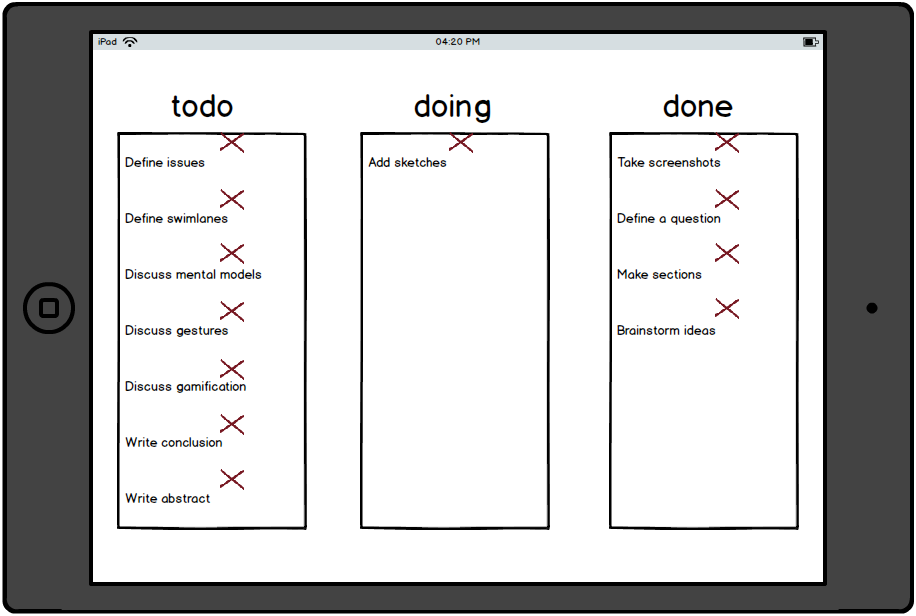
\includegraphics[scale=0.4]{images/mockup}}
    \caption{A simple mockup of the main functionality}   
    \label{figure:ipad-mockup}
\end{figure}

\begin{figure}[H]
    \centerline{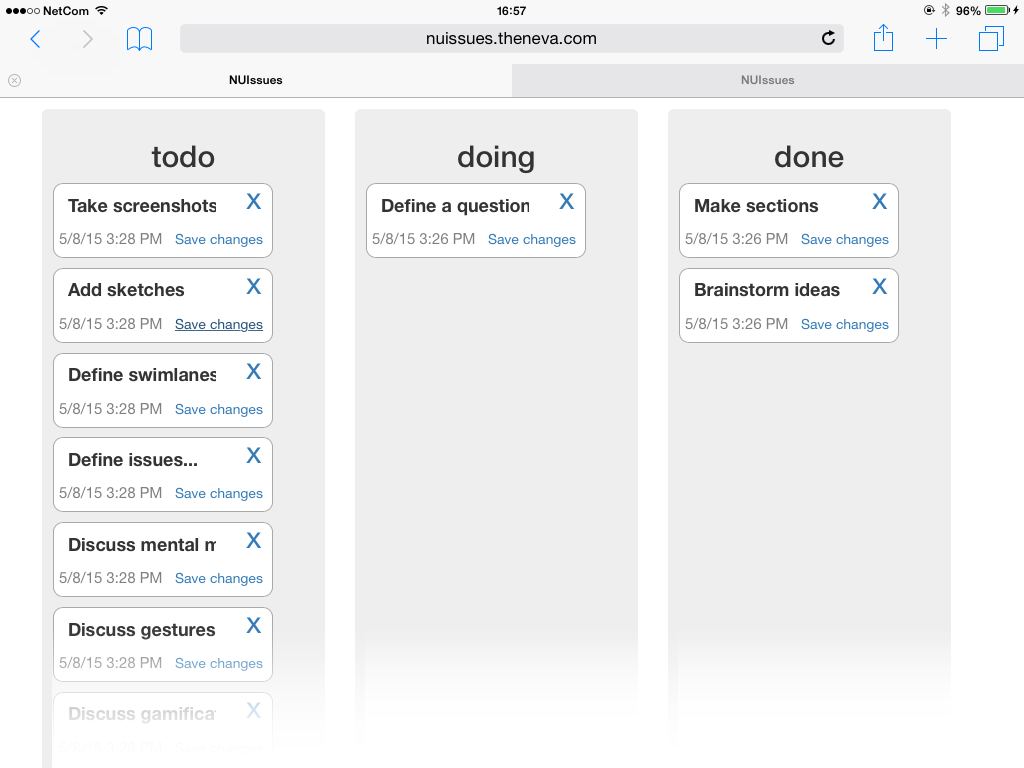
\includegraphics[scale=0.4]{images/nuissues-screenshots/01-default-all-swimlanes}}
    \caption{The system image for the main functionality}
    \label{figure:ipad-default-simple-screenshots}  
\end{figure}

NUIssues \textbf{only} supports \textit{touch} as natural input. While tracking changes on a user's skin and gaze tracking seem unrelated to the domain, there are several other to explore in future research: Gesture tracking, for instance, makes it possible to expand the application to run on interfaces like \textit{touch walls}. Adding speech recognition or building a Brain Machine Interface can be relevant if the system is to be used by people who are physically incapable of interacting with a touch interface. Of course, all new interface type implementations add to the complexity of the application and makes it harder to keep the GUI optimised for a single type like touch. There are also obvious development costs related to expanding the software.

The interface is designed only for Apple iPad 1/2/Mini, but one may easily write responsive CSS to support more types of devices. This allows bringing the very simple interface to natural interfaces like \textit{touch walls}, \textit{touch tables}, in addition to smartphones and desktop computers. The interface is designed to be used when sitting down, although the application can certainly merely be opened if the user's intent is to grok the project's state while on the move.

If the user intends to edit textual content (only the title in NUIssues), it would be preferable to have an external keyboard. As reflected upon in the introduction, a keyboard is by far the most effective tool to write precise text in a computer system. An on-screen software keyboard will work almost as well, but overlaps almost all of the issues. Thus, the application is unusable for anything other than finishing text input and saving changes when in the editing state.

The system is single-user, so inter-user task coupling \autocite[39]{wigdow-wixon:brave-nui-world:2011} has not been explicitly addressed, but it is possible to evolve the system to support other forms of interfaces like touch walls or touch tables (or even just real-time updates for a project). 

An issue that is not addressed in the proof of concept, but needs to be addressed in a full version of any issue tracking system is how one identifies users. In a touch-optimised system, it is preferable to avoid text input. Thus, one may look to how Apple identifies users on iPhone devices with fingerprint unlocks using a tangible user interface (TUI) \autocite{ishii-ullmer:tangible-bits-towards-seamless-interfaces-between-people-bits-and-atoms:1997}.

Any natural type of user recognition imposes hardware requirements on the devices that will run the application, but should be available as an option if they are viable for the organisation and target audience. Other natural forms of user identification include face recognition and speech recognition. A regular password option should be present, however.

Certain ethical concerns arise when identifying users. What can be stored on the device, what can be stored on a central server, and what should not be stored at all? Apple has already faced issues regarding their Touch ID system\footnote{\url{http://venturebeat.com/2014/12/28/chaos-computer-club-claims-it-can-reproduce-fingerprints-from-peoples-public-photos/}}, and these are questions for further research to answer.

As far as gamification goes, there are no elements in the current implementation of NUIssues. However, applying the Mechanics, Dynamics, and Aesthetics (MDA) framework \parencite[107]{wigdow-wixon:brave-nui-world:2011} to an issue tracker could be interesting, and very simple if one implements issue assignment to individual users. For example, the system could calculate points based on number of solved issues or their complexity, display a semi-permanent leaderboard, and give the users badges based on their performance and activities.

\subsection{Mental models in NUIssues}

\textcite{wilson-rutherford:mental-models-theory-and-application-in-human-factors:1989} introduces the notion of \textit{mental models} within Human-Computer Interaction (HCI), defined as any human's psychological representation (and implied expectations for) any given concept or object. A person will build a mental model for themselves, and for any object they interact with. They introduce a framework for the design phase of any computer system, with four distinctly different models at play.

First, one needs to define a \textit{target system}. In this case, the target system is the NUIssues system and interface.

Second, there is a \textit{conceptual model}, which is a very accurate psychological representation of exactly what the system does, usually held by an expert user or the designer themselves.

Fourth, the target system projects a \textit{system image}, which is the implementation of the the conceptual model. This is the basis for the next element: the user's mental model of the system.

Fifth, the \textit{user} immediately builds a mental model of the system of the system based on the \textit{system image}. This model is the basis for what the user expects the system to be able to do, mostly based on previous experience with similar systems but only based on the hints given by the application.

Last, the \textit{designer has a mental model of the user's model}, in which the designer attempts to guess what the user's mental model of the system image will be like.

The last model is built on the target audience's expected background, and can be built by considering similar applications the user can be expected to have interacted with in the past. In this case, an obvious system is that of sticky notes and checklists to track tasks, which almost everyone has used at some point. Thus, these graphical representations of issues may be used as metaphors in the system. Further, the user can have come across several digital issue trackers optimised for web like \footnote{\url{https://trello.com}}, Atlassian JIRA\footnote{\url{https://jira.atlassian.com/secure/Dashboard.jspa}}, Ding\footnote{\url{https://ding.io}}, ServiceNow\footnote{\url{http://www.servicenow.com/}}, and IBM Notes\footnote{\url{http://www-03.ibm.com/software/products/en/ibmnotes}}. Thus, using common, good metaphors and following best practises is important when designing a system for use (which is, indeed, \textit{any} system).

\subsection{Behaviour models}

\textcite{mackenzie:motor-behaviour-models-for-human-computer-interaction:2003} introduces the Hick-Hyman Law which considers (average) response time when dealing with multi-option menus, and the Keystroke-Level Model (KLM), which considers with the user's time to actually complete their task. These are not considered further as NUIssues is a very simple application with no menus and only two core functions that build on existing knowledge from using the tablet that runs the application. One relevant aspect from the KLM, however, is the system response time factor: if the application runs on a slow physical server, the entire system will feel sluggish and slow to the user. 

\textcite[4]{mackenzie:motor-behaviour-models-for-human-computer-interaction:2003} also introduces Buxton's \textit{3-state-model} for graphical input devices. While Buxton's model was defined for mouse interaction, the same "syntax" can be used to describe touch input. For example, in the scenario of dragging a card, the system has three states:

\begin{enumerate}
  \item State 0: No contact with input (screen) (idle). Enables entering state 1.
  \item State 1: Contact with card and moving (dragging). Lifting the finger off the card releases the card and sends the system back to state 0.
\end{enumerate}

\subsection{Development process}

NUIssues is developed as a web application with touch support, designed for an iPad 1/2/Mini. The question this project attempts to answer (how can optimising an issue tracker for touch boost productivity?) is not (very) concerned with different device sizes for the same device \textit{type}, so this was a simple way to prove the concept without complicating matters. Thus, the code base is rather clear -- but also very focused.

Of course, building a native application would give access to higher performance and complete control of the environment. However, native code is often more complicated and can not be easily expanded to support more than one operating system. Unlike native applications, web applications with mobile support can be run on all modern device types, including phones, tablets, and web browsers – and can potentially also be used on a touch wall or touch table interface as long as the software can run a web browser that can execute modern JavaScript.

No Software Development Kits (SDKs) specific to Natural User Interface design have been used, although the application leans on several frameworks and libraries commonly used in the MEAN (MongoDB, Express, AngularJS, Node.js) software stack:

\begin{itemize}
  \item AngularJS is used as a front-end Model-View-Controller (MVC) framework with support for communicating efficiently with a server,
  \item ng-sortable is an AngularJS module for building interactive lists with touch support -- in this case used to build the swimlanes,
  \item Bootstrap 3 is used together with custom CSS to give the application a well-tested base design,
  \item Node.js is a server runtime for JavaScript which runs the web server,
  \item Express is the web server which runs on Node.js,
  \item Mongoose is the Object-Document Mapper (ODM) that bridges Node.js and the MongoDB database (this project could just as easily have used relations, but documents are generally faster when working with JavaScript on the server),
  \item Body-Parser is used to convert JSON-formatted plain text to objects and back on the server, and finally
  \item MongoDB is the document database used to store issues
\end{itemize}

The front-end and back-end projects communicate using the Hypertext Transfer Protocol (HTTP) following the architectural style REpresentational State Transfer (REST). A sample implementation of creating an issue is implemented as follows:

Client-side service: \textbf{\textit{nuissues/angular/js/issues/issues.service.js}}
\begin{lstlisting}
service.create = function(issue) {
    return $http.post('/api/issues', issue);
};
\end{lstlisting}

Server-side controller exposing a REST endpoint: at HTTP POST <host>/api/issues\textbf{\textit{nuissues/node/controllers/issues.js}}
\begin{lstlisting}
router.post('/', function(req, res) {
	var issue = new Issue(req.body);
	issue.status = 'todo';
	issue.save(function() {
		return res.status(201).json(issue);
	});
});
\end{lstlisting}

Using the \texttt{ng-sortable}\footnote{\url{http://ngmodules.org/modules/ng-sortable}} module for AngularJS, the code for generating swimlanes in its entirety looks as follows where \texttt{validStatuses}, and \texttt{issues}, \texttt{swimlaneSortOptions} are defined by the page's AngularJS controller:

\begin{lstlisting}
<span id="board" ng-repeat="status in validStatuses">
    <div class="jumbotron swimlane">
        <h2>{{status}}</h2>
        <p ng-if="issues[status].length === 0">No issues!</p>
        <div as-sortable="swimlaneSortOptions" ng-model="issues[status]" class="pre-scrollable issue-list-container">
            <div class="issue-container" as-sortable-item ng-repeat="issue in issues[status]">
                <div as-sortable-item-handle ng-class="{issue: true, deleted: issue.deleted}">
                    <input class="title no-border" ng-model="issue.title" ng-change="issue.changed = true" ng-blur="issue.changed = true"/>
                    <span class="controls-delete">
                        <a ng-if="!issue.deleted" class="delete" href="javascript:void(0)" ng-click="issue.deleted = true">x</a>
                        <a ng-if="issue.deleted" class="restore" href="javascript:void(0)" ng-click="deleteIssue(issue)">✓</a>
                    </span>
                    <div class="created static">{{issue.created | date: 'short'}}</div>
                    <!-- <a ng-if="issue.changed" href="javascript:void(0)" class="control-update" ng-click="updateIssue(issue)">Save changes</a> -->
                    <a href="javascript:void(0)" class="control-update" ng-click="updateIssue(issue)">Save changes</a>
                </div>
            </div>
        </div>
        <div id="bottom-fade"></div>
    </div>
</span>
\end{lstlisting}

This code also shows the HTML implementation of the fade-out effect at the bottom of each swimlane, which is simply a \texttt{div} element styled with CSS as follows, assuming the file \texttt{bottom-fade.png} exists in the same directory as the CSS file (technique inspired by \url{https://css-tricks.com/examples/FadeOutBottom/}):

\begin{lstlisting}
#bottom-fade {
	width: 600px;
	height: 200px;
	z-index: 99;
	position: fixed;
	bottom: -20px;
	background: url("bottom-fade.png") bottom center no-repeat;
}
\end{lstlisting}

The live application is hosted on Heroku\footnote{\url{https://heroku.com}}, which is a free host for Node.js (and other) projects.

\subsection{Known bugs in the current implementation}

There is at present time one known bug in the prototype implementation:

\begin{itemize}
  \item It is nearly impossible to grab the bottommost issue that lies beneath the "fade out" overlay over the swimlane in a full swimlane
\end{itemize}
